\documentclass{article}
\usepackage{graphicx}
\usepackage{hyperref}

\title{Physics}
\author{}
\date{}

\begin{document}

\maketitle

\section{Models}
\begin{itemize}
\item VAE/CVAE  - P/A

%Prathyusha
After going through \cite{NIPS2015_8d55a249} paper, CVAE and its variants are trainable efficiently in the SGVB framework, and introduce novel strategies to enhance the robustness of the models for structured prediction. archtiecture layers dimensions 
%Prathyusha

% Amir
After working on \cite{kingma2013auto} paper and code, it was basically an auto-encoder which was try to reconstruction some handwriting. First I ran a cVAE for our problem. This cVAE were in two version. In the first version I used the momenta as condition and in the second version I used atomic masses as the condition. Then I try to run a VAE. The results ( we compared model based on loss function which was MSE + KLD) were better for a simple VAE without any condition. After that I tried to read the \cite{shmakov2024end} paper, to see what are the Conditions and how can we use CVAE and what can we use as the condition. We had a meeting with Prof. Caragea about Parton Data, Detector Variables, kinematics, missing transverse momentum (MET) and other data in the paper but we couldn't get to a good understanding of the problem so maybe the Physics department could help us regarding this paper or they could provide us some better data to use as condition.
In the Section~\ref{sec:Codes} there are details about these implementations.
% Amir

\item (C)INN  - P
In the paper \cite{Bellagente_2020} invertible neural networks are used for solving the inverse problem, yet to explore the MMD loss function as an add-on to MSE reconstruction loss, CINN is conditioned on detector features with coupling blocks.
\item VDM - A 

% Amir
I read and run the modified code of the paper \cite{kingma2021variational}. This paper is originally using images. The model is basically described in Figure~\ref{fig:vdm-diagram}.
\begin{figure}
    \centering
    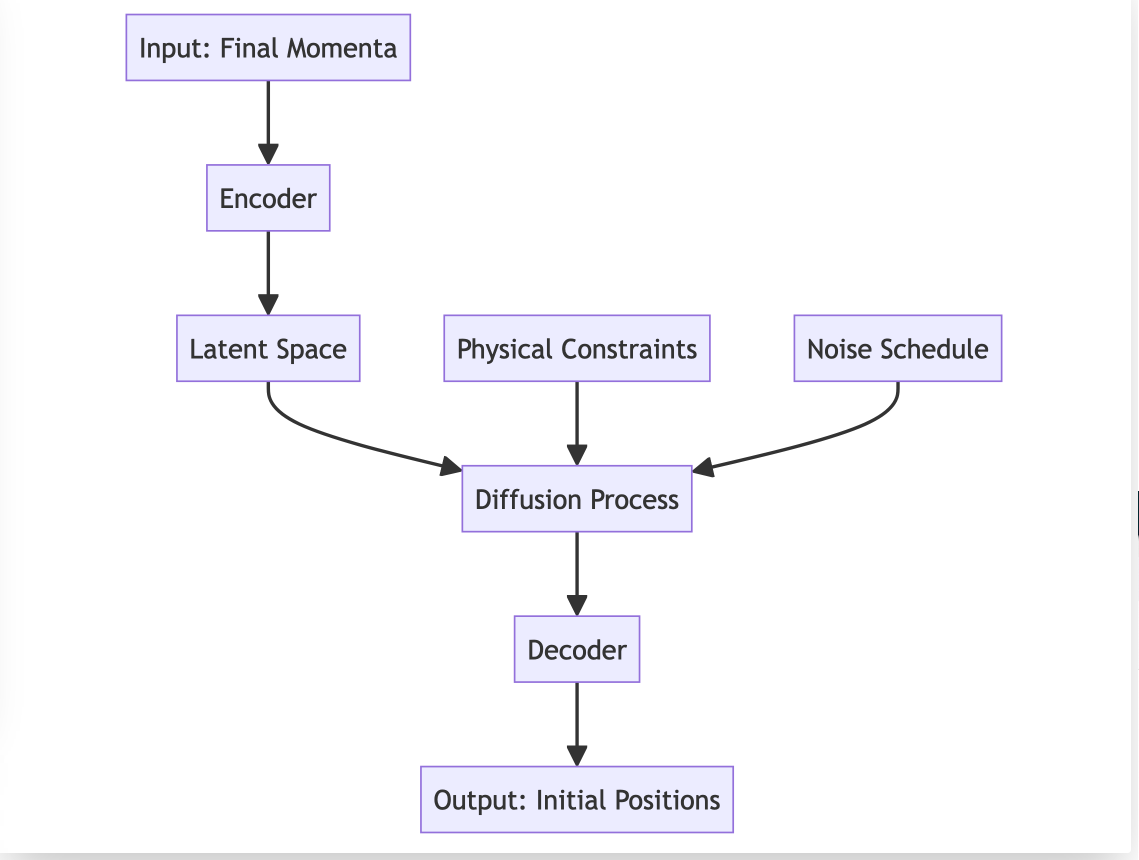
\includegraphics[width=10cm]{vdm-diagram.png}
    \caption{VDM Diagram}
    \label{fig:vdm-diagram}
\end{figure}
\\

I tried to implement this model using both Pytorch and Jax libraries. The main code of \cite{kingma2021variational} were written by Jax then I used an unofficial GitHub repository which used Pytorch to implement VDM. More explanation about this is in Section~\ref{sec:Codes}.


% Amir
\item LDM - P
In paper \cite{shmakov2024end} for Latent diffusion model, involves a parton encoder and parton decoder,detector encoder \cite{shmakov2024end} yet to explore on how to implement the physics informed consistency loss

\item VLD - A

% Amir
In the paper \cite{shmakov2024end}, they try something new as a better proposed model. Variational Latent Diffusion (VLD) is a unified method that combines the capabilities of latent diffusion models and variational diffusion models. It integrates the conditioning encoder, data VAE (Variational Autoencoder), and diffusion process into a single loss function.

The inputs and outputs are Parton Data and the conditions are Detector Variables. It's shown in below figure.

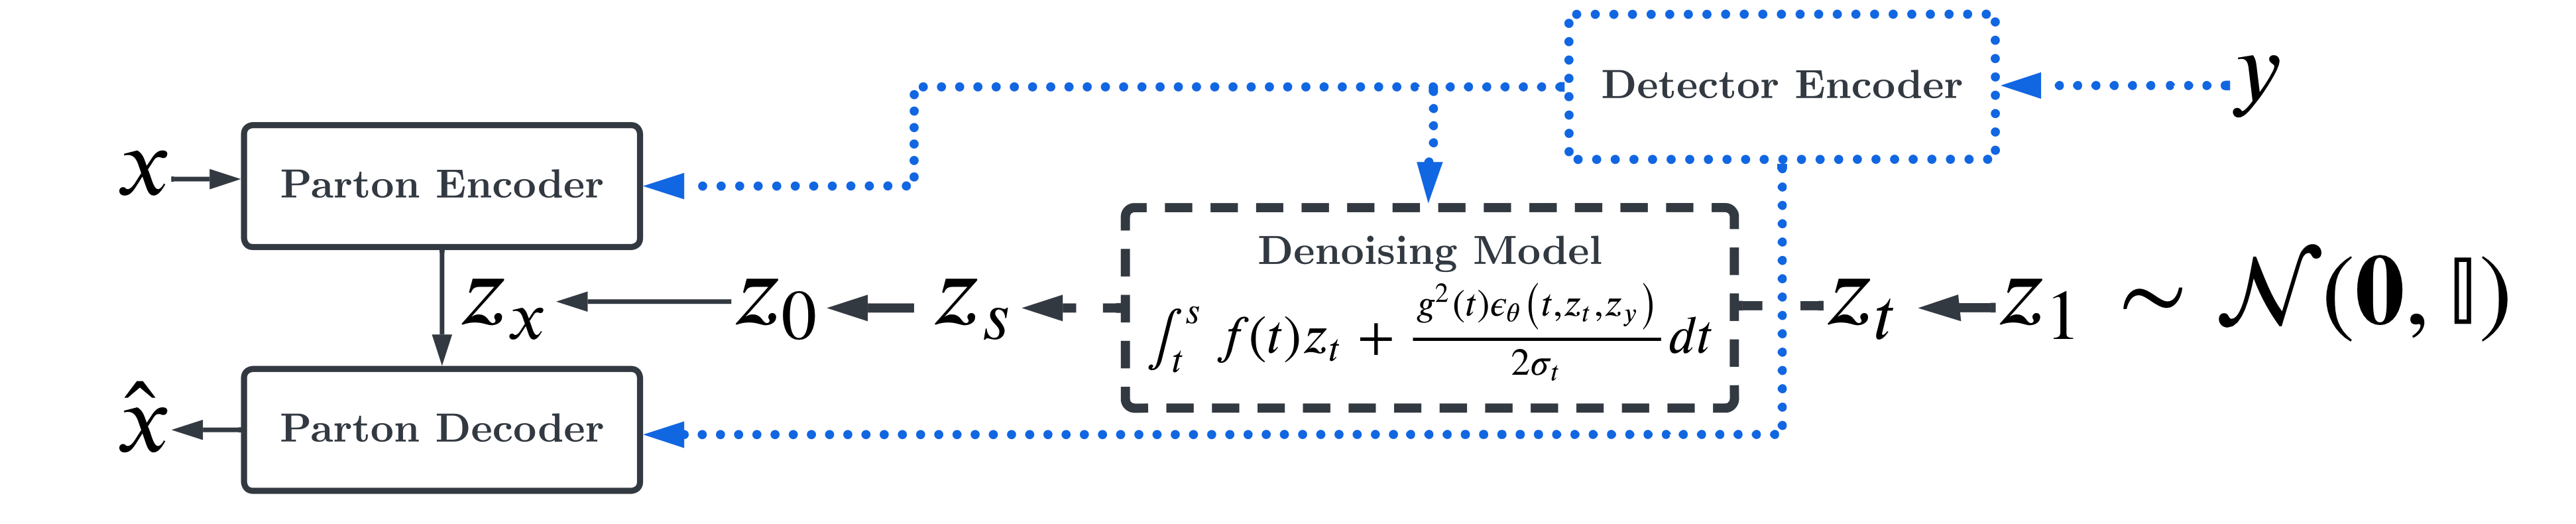
\includegraphics[width=10cm]{VLD.png}
% Amir
\end{itemize}

\section{Codes}\label{sec:Codes}
\begin{itemize}
\item VAE/CVAE  - P/A

% Amir
Some other refrences to this models are: \href{https://colab.research.google.com/github/lschmiddey/fastpages_/blob/master/_notebooks/2021-03-14-tabular-data-variational-autoencoder.ipynb#scrollTo=U70AsP_Cgf3v}{link1},\href{https://github.com/sfme/RVAE_MixedTypes}{link2},\href{https://github.com/unnir/cVAE}{link3}. To have a better understanding of how a CVAE works, I used \href{https://www.analyticsvidhya.com/blog/2023/09/generative-ai-conditional-vaes/}{link3} article code and try to run and print the model's summary. It's summary in addition to some of the important parameters are shown as Figure~\ref{cVAE-Summary}.
\begin{figure}
    \centering
    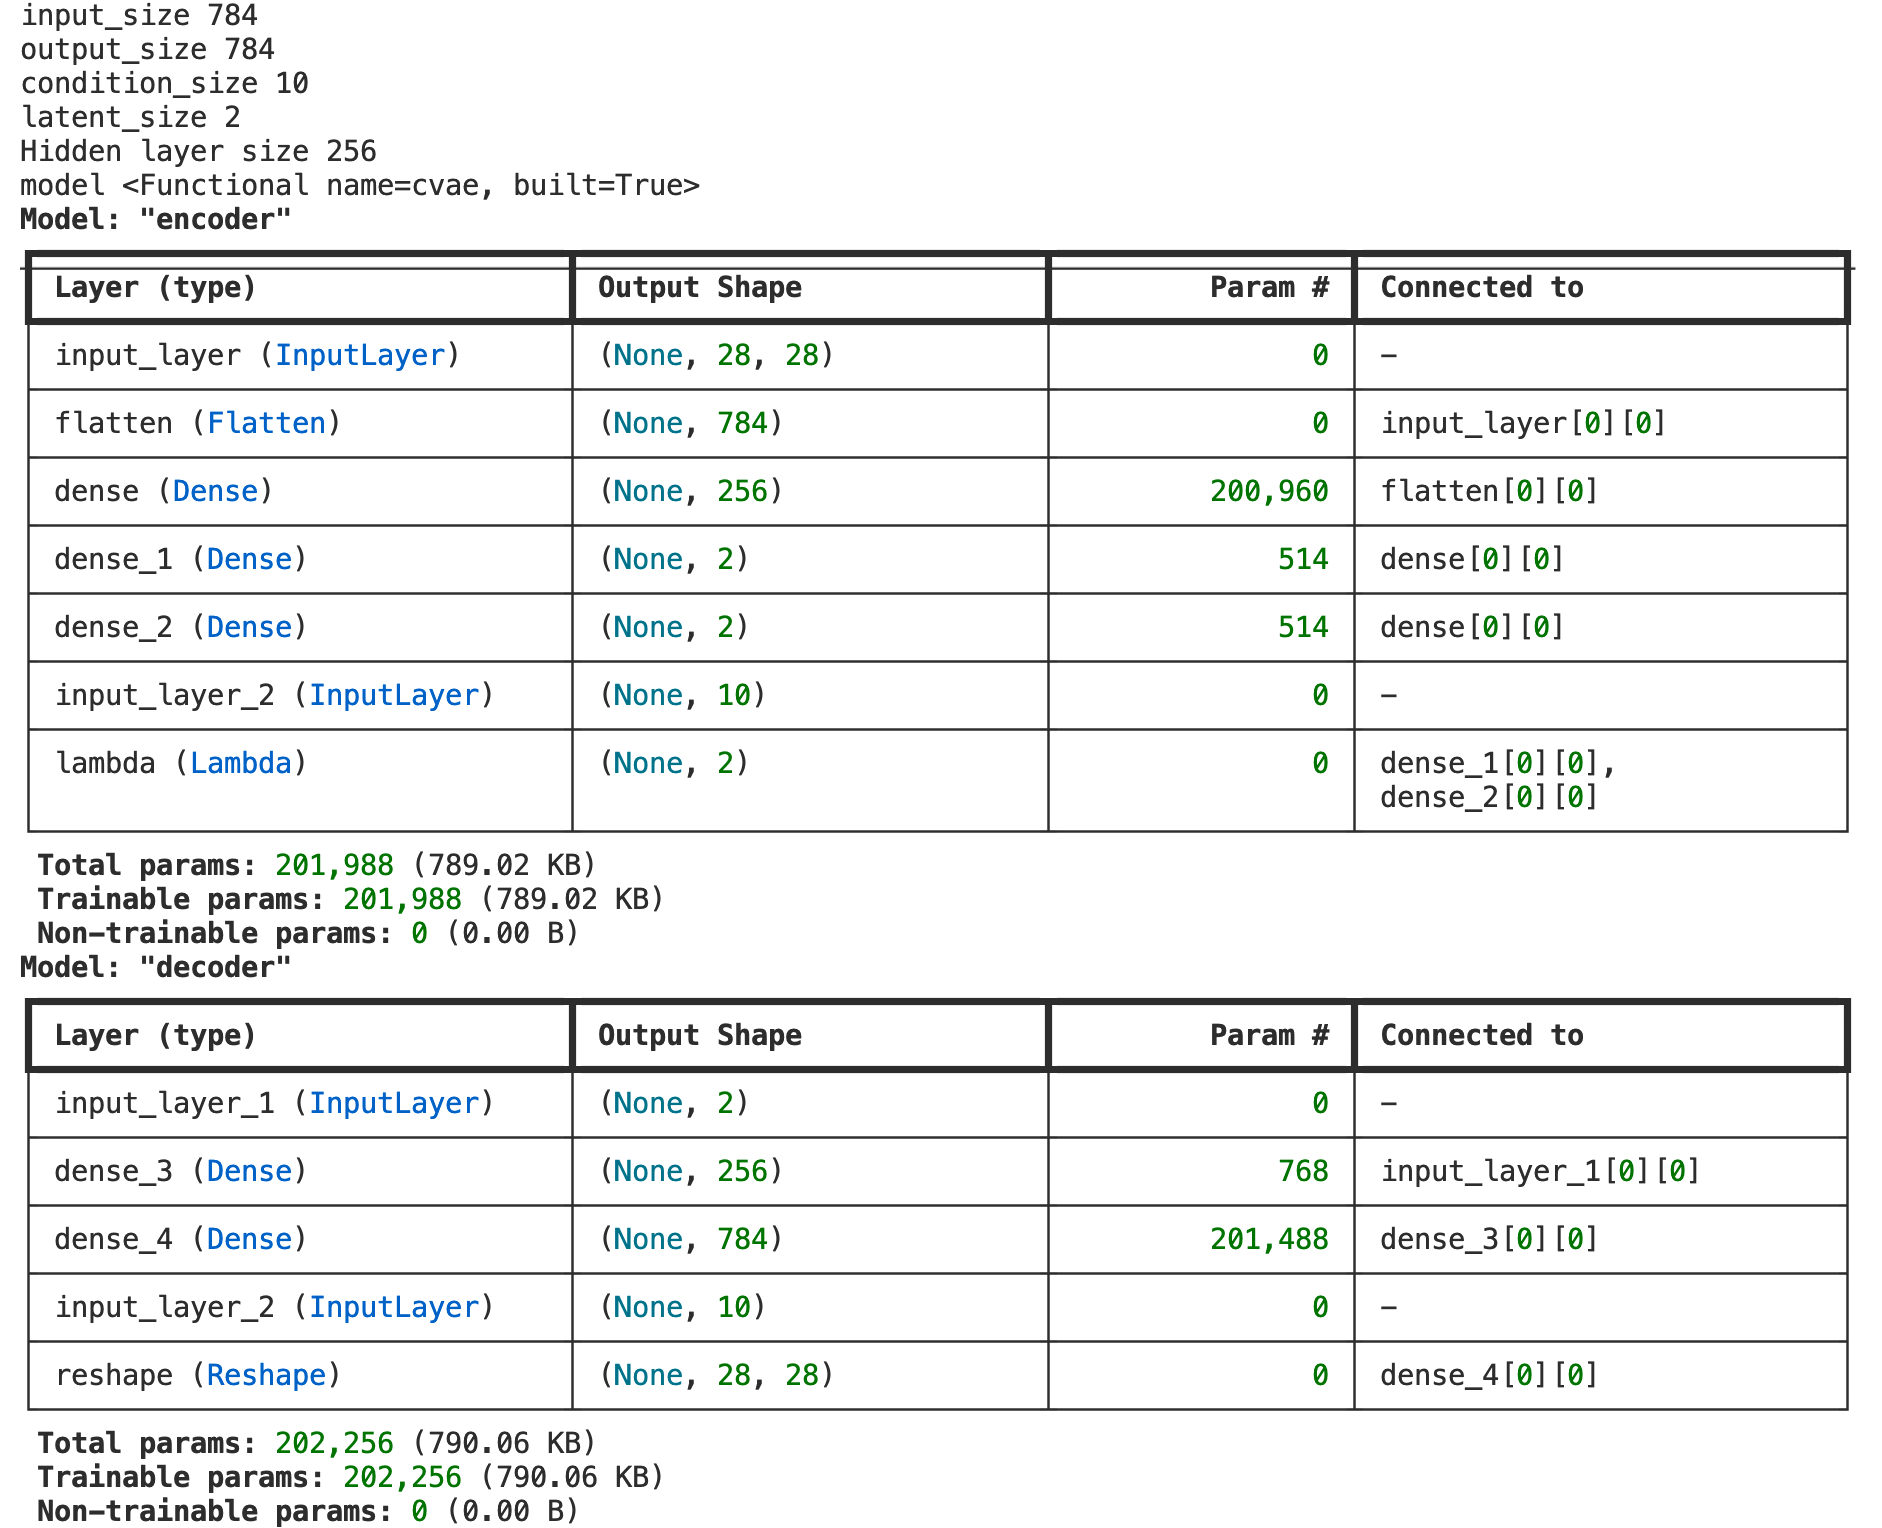
\includegraphics[width=10cm]{Summary1.png}
    \caption{cVAE-Summary}
    \label{cVAE-Summary}
\end{figure}



Also in the article they illustrated some architecture for the above autoencoder which is presented in Figure~\ref{cVAE-Architecture}. Label Y is considered as the condition in this architecture.
\begin{figure}
    \centering
    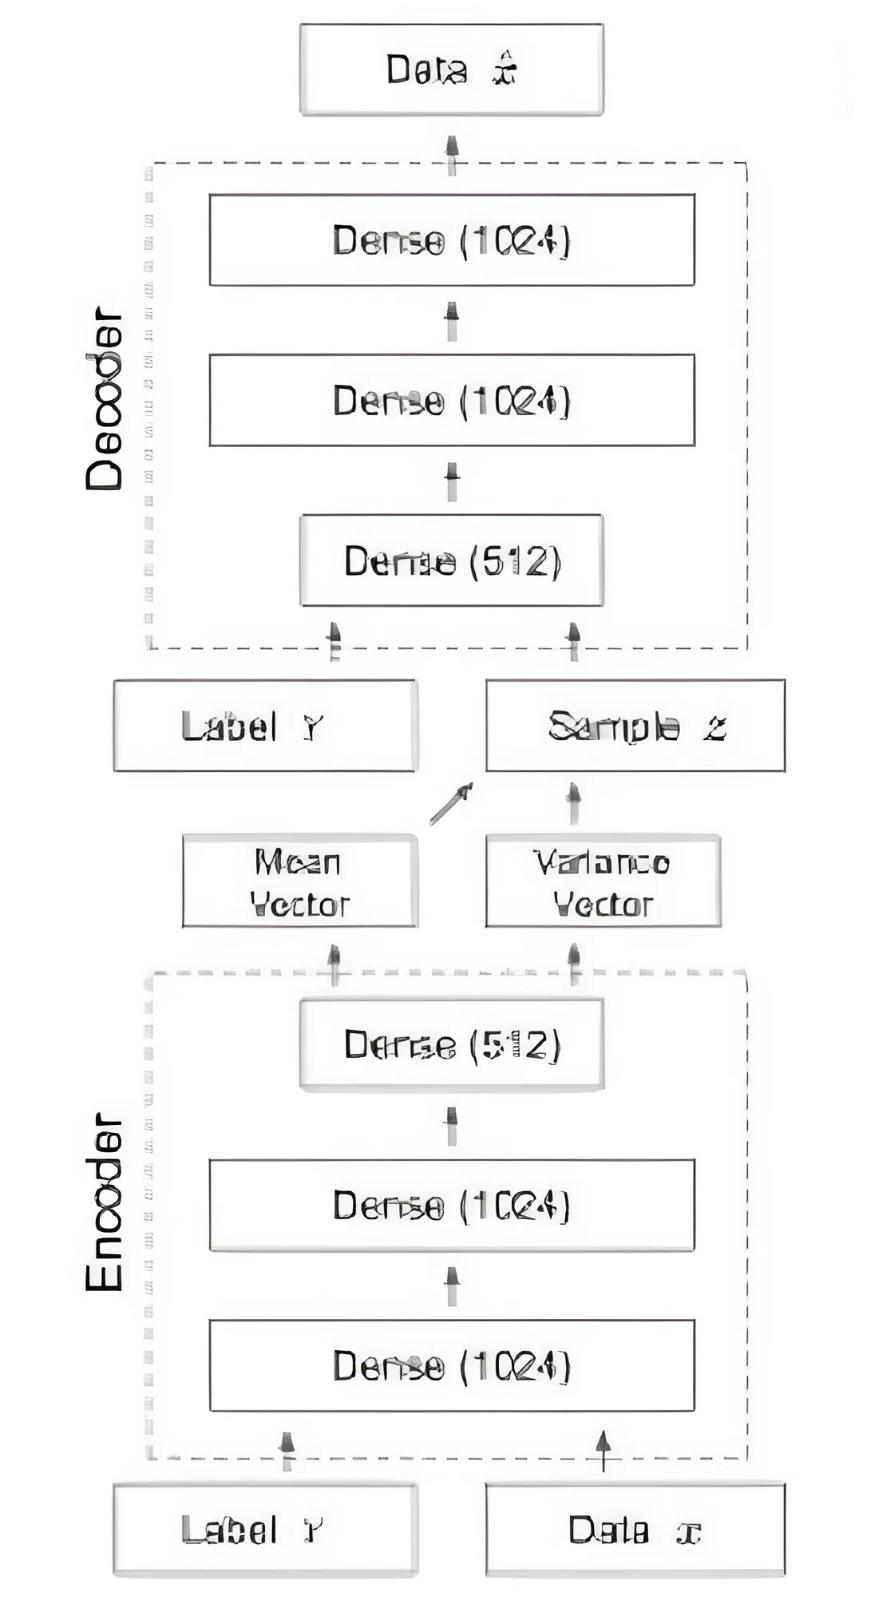
\includegraphics[width=3.8cm]{Architecture1.png}
    \caption{cVAE-Architecture}
    \label{cVAE-Architecture}
\end{figure}


The codes are available in \href{https://ksuemailprod-my.sharepoint.com/:f:/g/personal/ghanaatian_ksu_edu/EtM8nGAp84lPpl0hEyB99BABTLVZoLJScyU0aYGzuPtY5A?e=cRbT5P}{cVAE-Codes}
\\
% Amir

%Prathyusha
The reference \href{https://github.com/ucals/cvae}{code} used for CVAE 

The important parameters of the CVAE executed

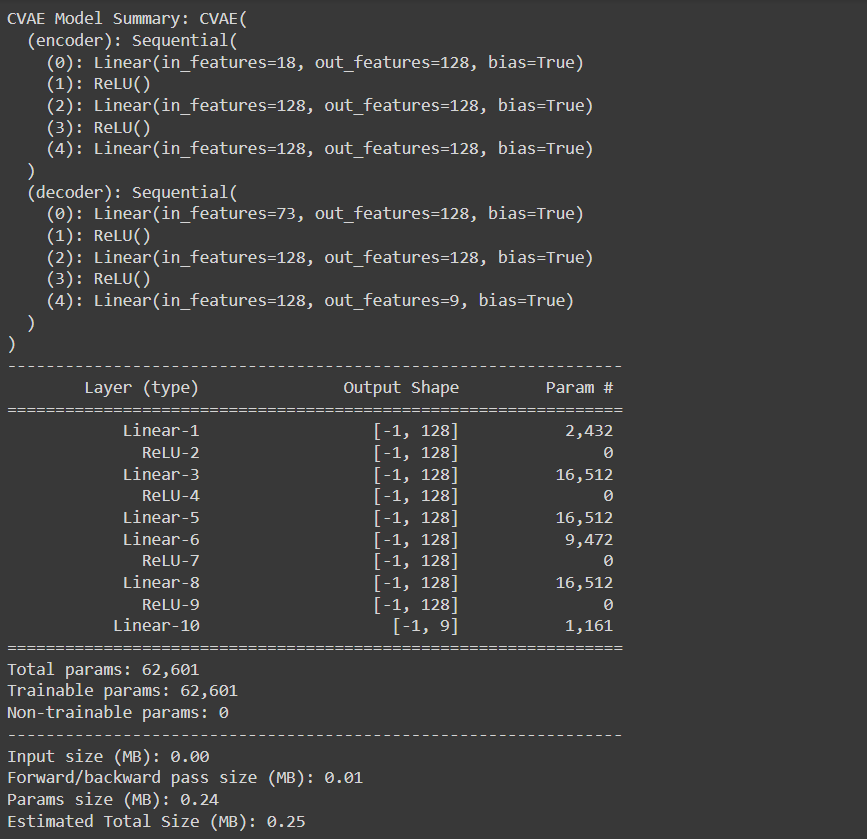
\includegraphics[width=10cm]{Screenshot 2024-06-12 130407.png}

VAE
Basic Encoder and decoder are executed and the parameters are 

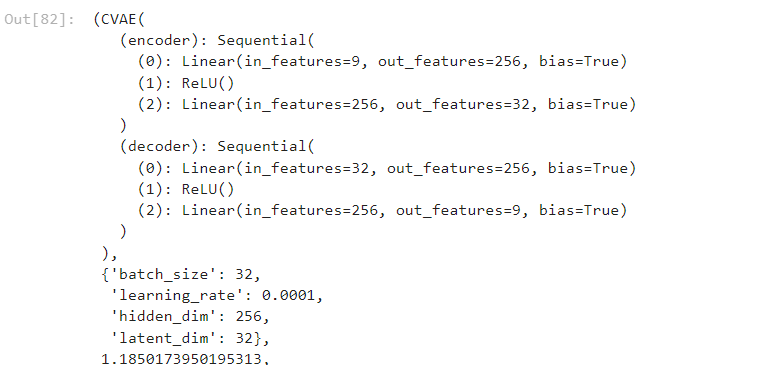
\includegraphics[width=10cm]{Screenshot 2024-06-12 133437.png}
%Prathyusha

\item VDM - A

% Amir
The code for this model is on this Github repository: \href{https://github.com/google-research/vdm?tab=readme-ov-file}{link1}.
The code from Google, doesn't use Pytorch so I found several pythorch implementation of VDM on github such as \href{https://github.com/DavidRuhe/simple-variational-diffusion-models?tab=readme-ov-file}{link2} and \href{https://github.com/addtt/variational-diffusion-models?tab=readme-ov-file}{link3}.
I was able to run the VDM code with pytorch from the github repository. The codes are available in \href{https://ksuemailprod-my.sharepoint.com/:f:/g/personal/ghanaatian_ksu_edu/ErHzoMrrgF5JplZ5MKVOfI8BHHcqv4EBVr75vvKSQKCxCw?e=s2DnMd}{VDM-Codes}. With same normalization (only on the input), the final loss value for VAE is about 0.4856 and for VDM is 1.8968 (after doing the hyperparameter optimization).
% Amir
\item LDM - P
The code involves references from .zip file released by this paper \cite{shmakov2024end}, But I am not sure regarding the loss function
%P
The code for this model is 
%P
\item UC-VLD - A $->$ inputs/outputs

% Amir
The code for this model is on this Github repository: \href{https://openreview.net/forum?id=v7WWesSiOu}{link1}. These models are variations on the proposed unified Variational Latent Diffusion (VLD) architecture. They correspond to an unconditional VAE (VLD), a conditional encoder and decoder (C-VLD), or a conditional encoder with an unconditional decoder (UC-VLD). There's no specefic code for VLD in the codes.
% Amir

\item Simple Encoder-Decoder - A

% Amir
After training the VAE and VDM model, I tried to create a simple Encoder-Decoder architecture and a MSE loss function and without doing any normalization the result was better, the attached file is its python script. I think maybe because of the low amount of data for training  (800 rows without considering validation set) a simple architecture works better as we only have 9 inputs and 9 outputs.The codes are available in \href{https://ksuemailprod-my.sharepoint.com/:f:/g/personal/ghanaatian_ksu_edu/EoOYzAEZjGNHj3JdlJOCs50Br5Qrd0Ns81kRbANULvxrzQ?e=ZucWfZ}{ED-Codes}
% Amir
\end{itemize}

\section{Final VAE} %Amir

The VAE-4th model was trained and tested with the 1 Million rows dataset. Using a VAE model, the model hyper-parameters were all fine-tuned and then I tested Mean Square Error, R-Squared and Mean absolute error with the 10,000 rows dataset. I've saved the model and the code is available to explore and test random rows of momenta to predict its initial positions! 

Figure \ref{fig:testcases} shows some test cases with the value of the mentioned Errors. Figure \ref{fig:realvspredicted} shows for each of 9 positions how predicted values are compared to the real values in a visual approach as blue points are real values and red points are predicted. Also, there's a Learning curve plot which is being shown in Figure \ref{fig:learningcurve}.

\begin{figure}[h]
    \centering
    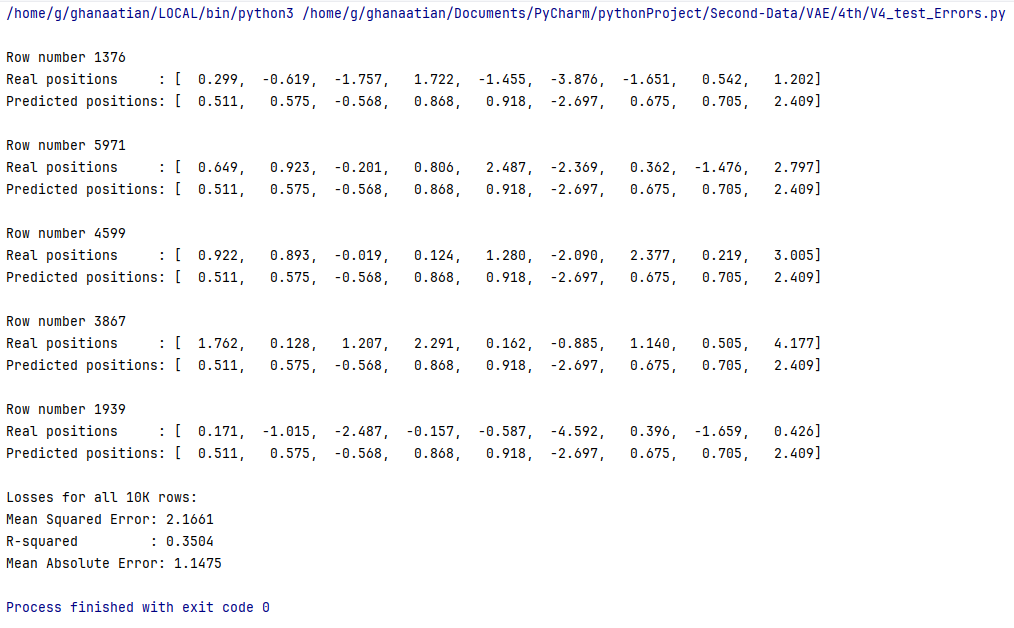
\includegraphics[width=0.8\textwidth]{VAE4th-testcases.png}
    \caption{Test cases with Error values}
    \label{fig:testcases}
\end{figure}

\begin{figure}[h]
    \centering
    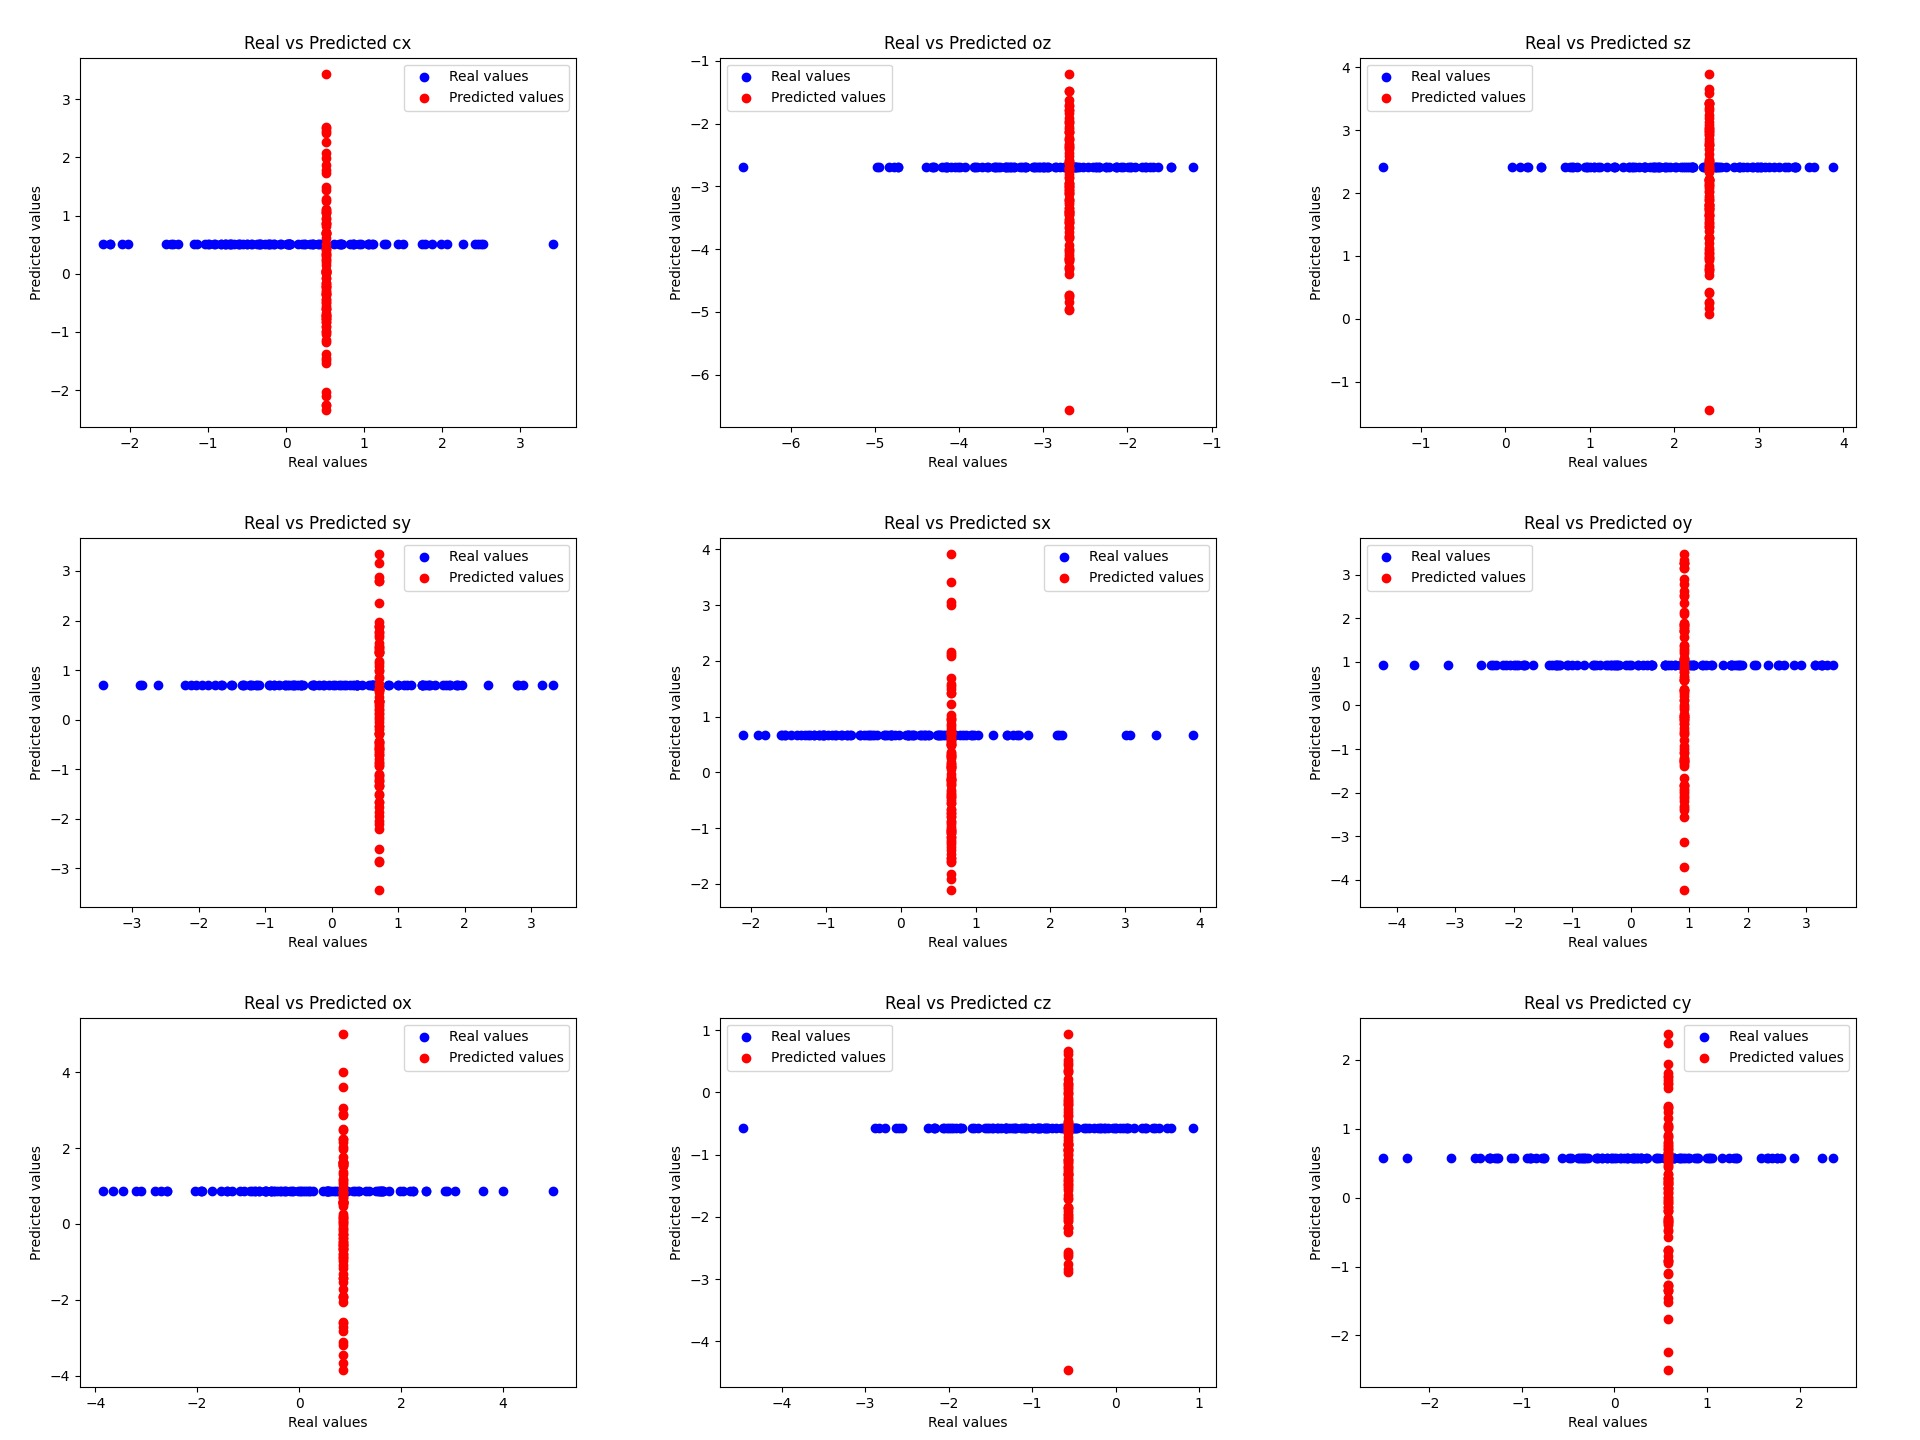
\includegraphics[width=0.8\textwidth]{VAE4th_REALvsPREDICTED.png}
    \caption{Real vs Predicted values for 9 positions}
    \label{fig:realvspredicted}
\end{figure}

\begin{figure}[h]
    \centering
    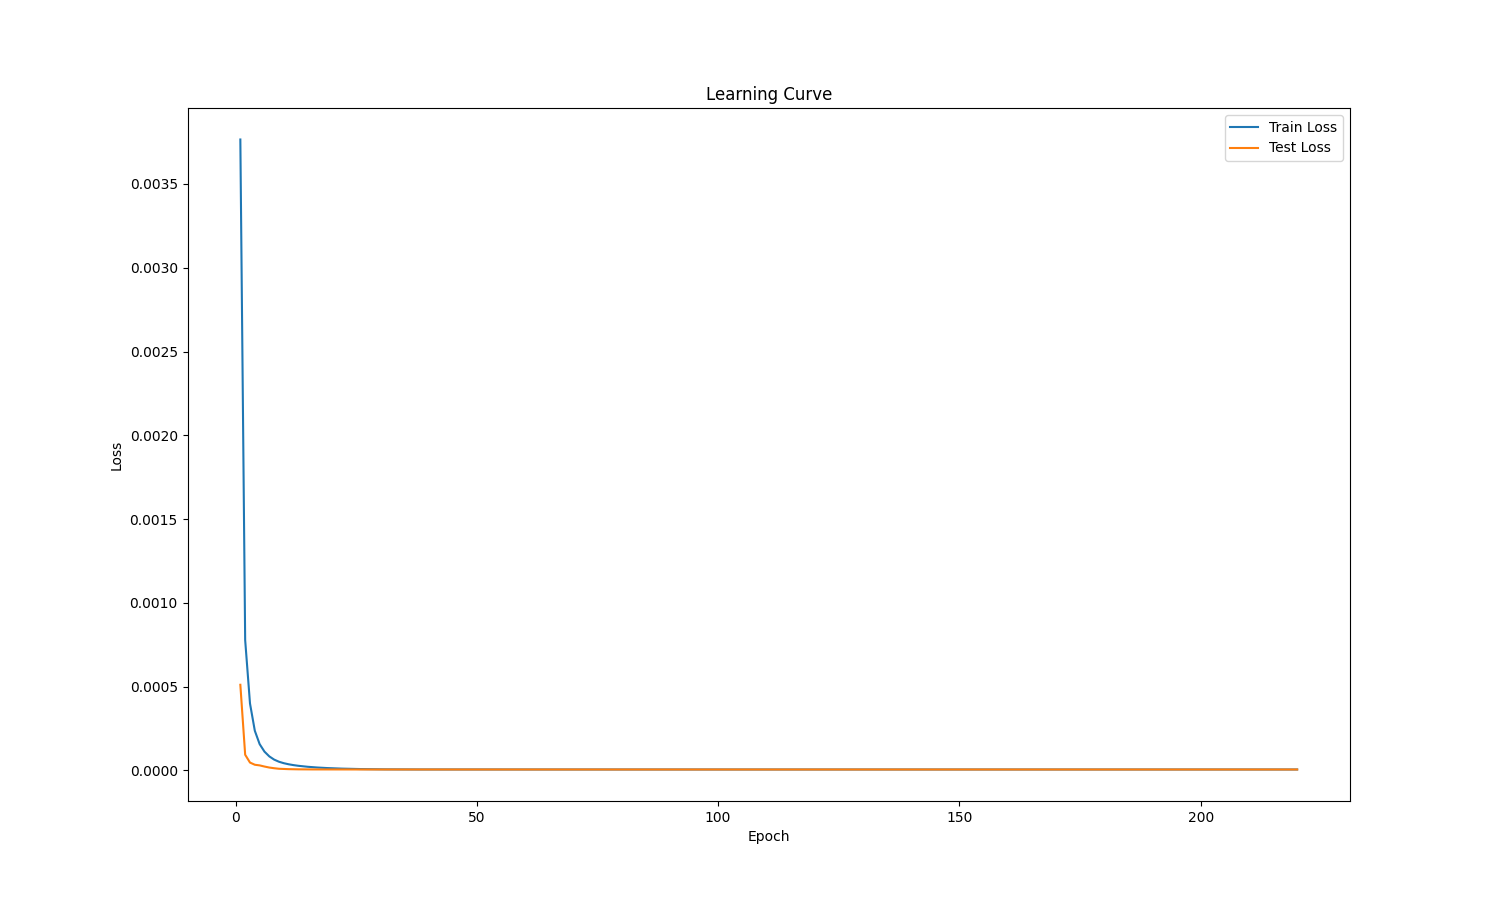
\includegraphics[width=0.8\textwidth]{VAE4thlearning_curve.png}
    \caption{Learning curve plot}
    \label{fig:learningcurve}
\end{figure}

Below issues were also evaluated to get a better model:

\begin{enumerate}
    \item Hyperparameter Tuning
    \item Using MinMaxScaler
    \item Changing Network Depth and Width:
    \begin{itemize}
        \item Increase the number of layers and neurons in both encoder and decoder.
        \item Experiment with different architectures, gradually increasing complexity.
    \end{itemize}
    \item Activation Functions: Replace ReLU with LeakyReLU or ELU in the VAE class.
    \item Dropout: Add dropout layers to prevent overfitting.
    \item Adjust the gradient clipping max norm. values between 0.1 and 5.0
    \item Add L2 regularization to the code. L2 regularization, also known as weight decay, is a common technique to prevent overfitting by adding a penalty term to the loss function based on the magnitude of the model's weights.
    \item Implement more comprehensive evaluation metrics beyond MSE, such as R-squared or Mean Absolute Error.
    \item Visualize predictions vs. actual values to identify patterns in errors.
\end{enumerate}

The attachment (\href{https://ksuemailprod-my.sharepoint.com/:f:/g/personal/ghanaatian_ksu_edu/Ek_s1HBx0yRNpPJa34HqJGoBzaNhzVutGev2CZHL_IE_yA?e=fcbfwg}{link}) contains a python script that generates five random predicted rows (positions) with the saved model. You could simply run the python script if you have all the libraries installed and there's no need to change anything in the code.


\bibliographystyle{unsrt}
\bibliography{references} 
\end{document}
